\documentclass{beamer}
%pacchetti
\usepackage[T1]{fontenc}
\usepackage[utf8]{inputenc}
\usepackage{graphicx}
\usepackage[italian]{babel}
\usepackage{mathrsfs}
\usepackage{booktabs}
\usepackage{amsmath}
\usepackage{amsfonts}
\usepackage{amssymb}
\usepackage{amsbsy}
\usepackage{amsthm}
\usepackage{enumerate}
\usepackage{quoting}
\quotingsetup{font=small}
\usepackage{diagbox}
\usepackage{graphicx}
\usepackage{setspace}
\usepackage{float}
\usepackage{version}
\usepackage{multicol}
\usepackage{beamerfoils}

\usepackage[none]{hyphenat} %avoid hyphenation
\usepackage{xcolor} %to uset \textcolor
\usepackage{bbm} %funzione indicatrice
% end pacchetti

\usetheme[bgphoto]{polimi}

% Full instructions available at:
% https://github.com/elauksap/beamerthemepolimi

% Set custom font (requires to compile with XeLaTeX).
\usepackage{ifxetex}
\ifxetex
\usepackage{fontspec}
\setsansfont[Scale=0.9]{Arial}
\fi

\usepackage{lipsum}


\newcommand\mynum[1]{%
	\usebeamercolor{enumerate item}%
	\tikzset{beameritem/.style={circle,inner sep=0,minimum size=2ex,text=enumerate item.bg,fill=enumerate item.fg,font=\footnotesize}}%
	\tikz[baseline=(n.base)]\node(n)[beameritem]{#1};%
}


\title{Coupled Markov chains with applications to Approximate Bayesian Computation for model based clustering}
%\subtitle{Subtitle}
\author{E. Bertoni, M. Caldarini, F. Di Filippo, G. Gabrielli, E. Musiari}
\date{10 January 2022}


%Cose da fare

% Mettere biografia
% Mettere \pause e colori
% Sistemare il titolo e layout

\begin{document}

\begin{frame}
\maketitle
\end{frame}

\begin{section}{Introduction}

	\begin{frame}
		\frametitle{A complex problem}

 		\begin{minipage}{0.45\textwidth}
 			\begin{center}
 				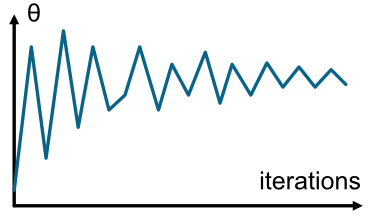
\includegraphics{img/markov_singola}
 			\end{center}
 		\end{minipage}
 		\hfill
 	 	\begin{minipage}{0.45\textwidth}
 	 		\begin{center}
 	 				
\includegraphics{img/likelihood_na}
 	 		\end{center}
 		\end{minipage}
 		
 		\vspace{0.5cm}

 		\begin{minipage}{0.45\textwidth}
 			\begin{center}
 				$\Downarrow$

 				\textbf{Unbiased Markov chain Monte Carlo methods with couplings}
 			\end{center}
 		\end{minipage} %}
 		\hfill
	 	\begin{minipage}{0.45\textwidth}
 			\begin{center}
 				$\Downarrow$
 				
 				 \textbf{Approximate Bayesian Computation}
 			\end{center}
 		\end{minipage} %}
 	 	
 	 	\vspace{0.2cm}
 	 	
 	 	\begin{minipage}{0.45\textwidth}
 	 		\begin{center}
 	 			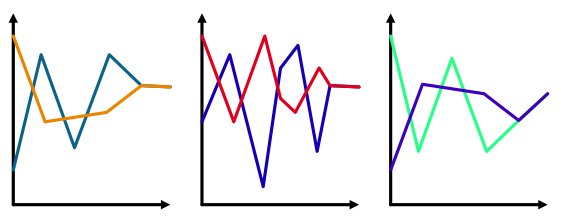
\includegraphics{img/markov_coupled_parallel}
 	 		\end{center}
 	 	\end{minipage}%}
 	 	\hfill
 	 	\begin{minipage}{0.45\textwidth}

 	 	\end{minipage}
 	 	
 	 	
 	 	
	\end{frame}

\end{section}



\begin{section}{Unbiased Markov chain Monte Carlo methods with couplings}
	\begin{frame}[plain]{}
		\sectionpage
	\end{frame}

	\begin{frame}
		\frametitle{Structure of the method}
		\begin{center}
			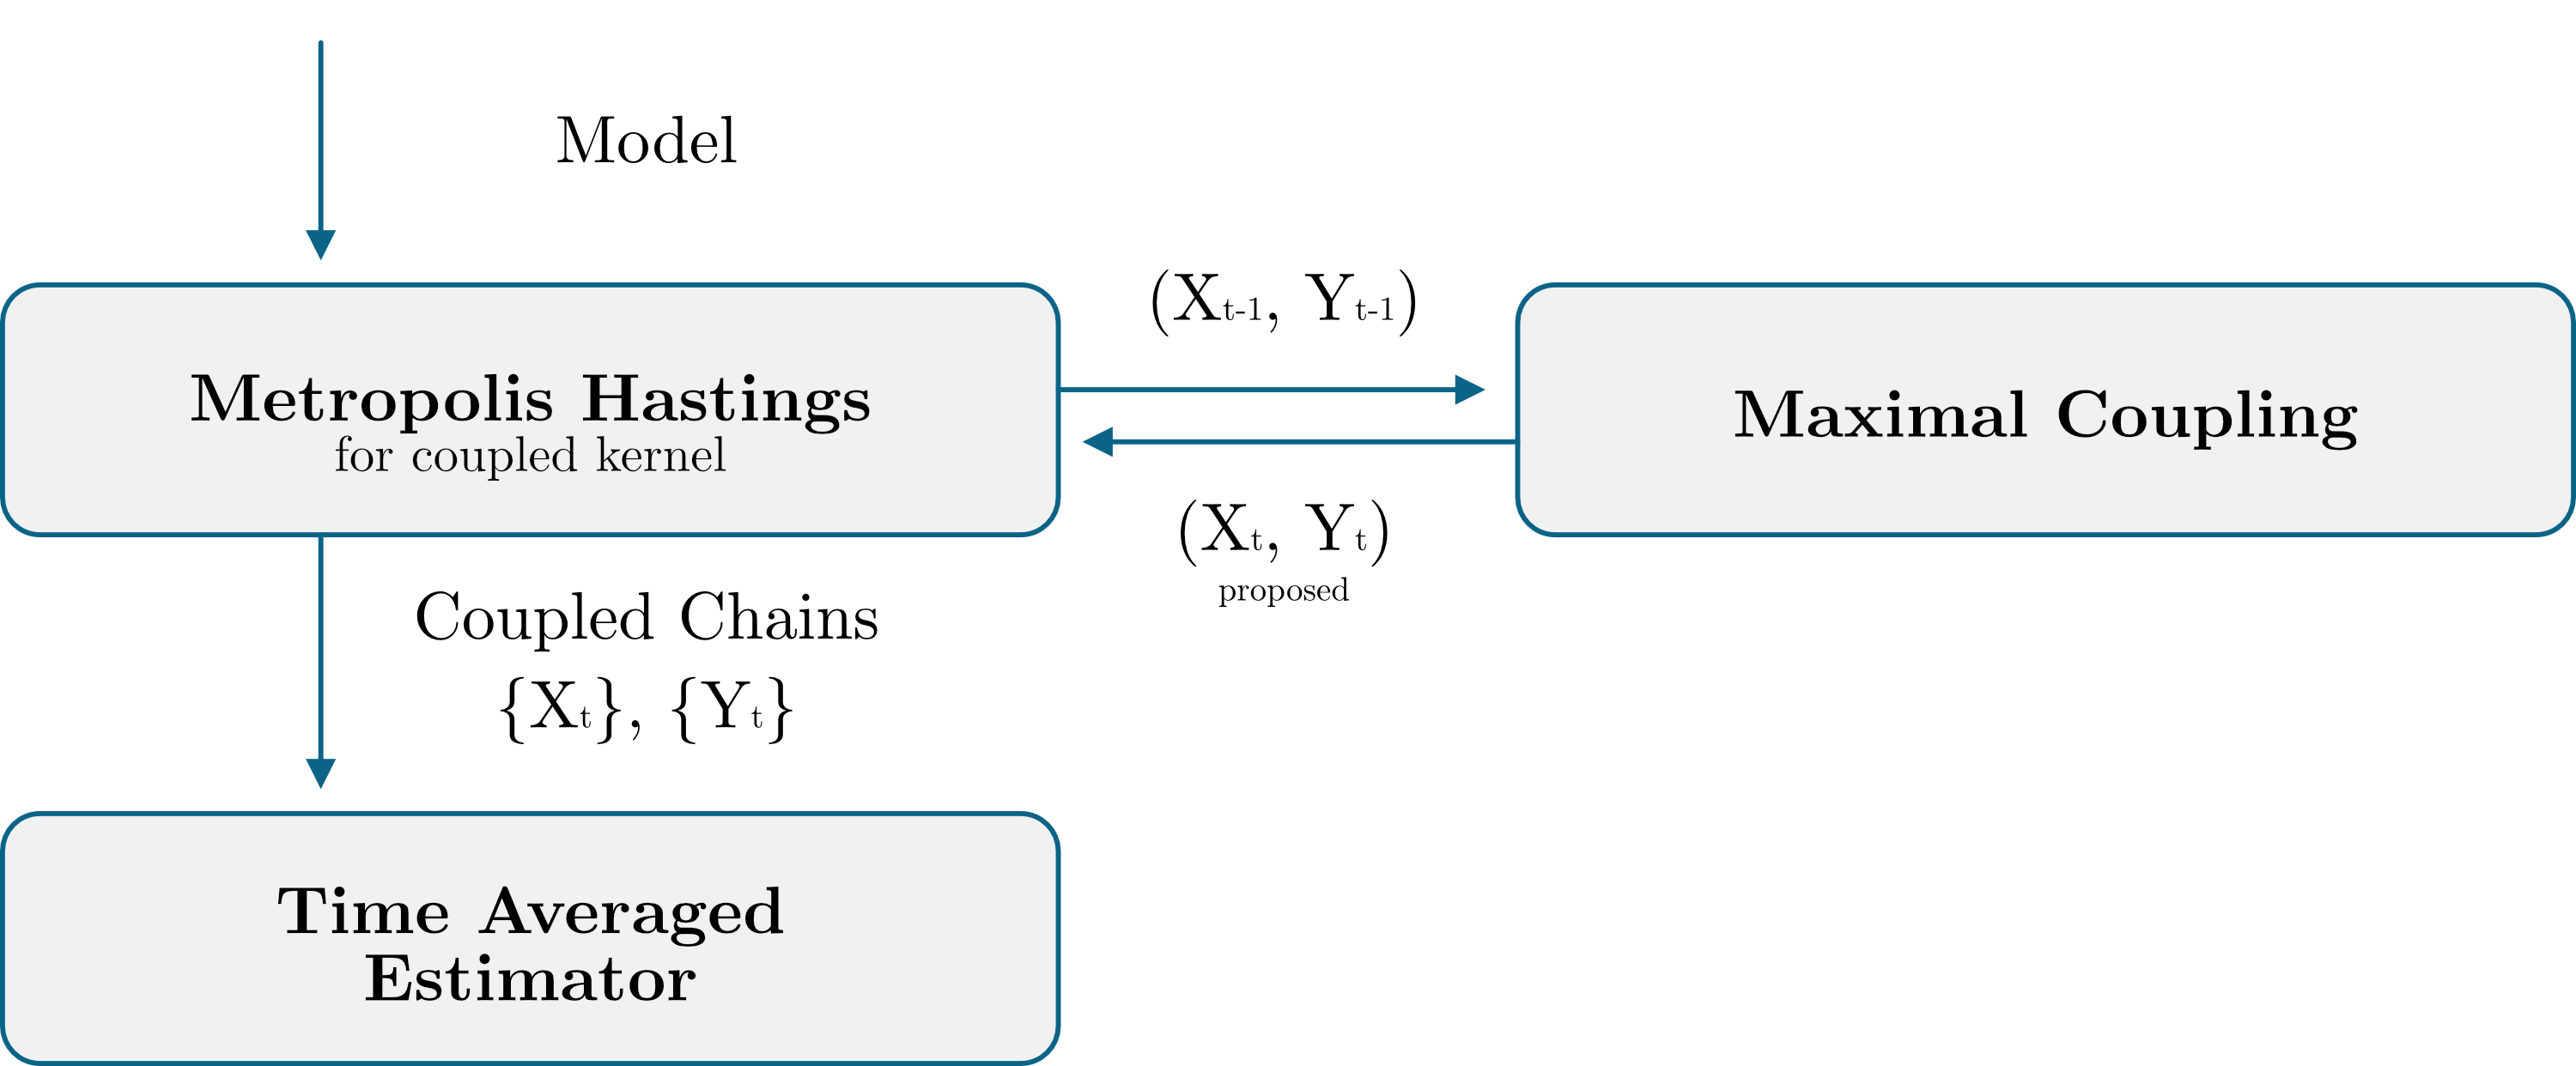
\includegraphics[width=0.95\textwidth]{img/Bayes1}
		\end{center}
	\end{frame}
	
	\begin{frame}
		\frametitle{Time-averaged estimator}
		\begin{enumerate}
			\item draw $X_0$ and $Y_0$ from an initial distribution $\pi_0$ and draw $X_1 \sim P(X_0, \cdot)$;
			\item set $t=1$: while $t<\max\{m,\tau\}$ and:
			\begin{itemize}
				\item[a] draw $(X_{t+1}, Y_t)\sim \bar P \{(X_t, Y_{t-1}), \cdot \}$; 
				\item[b] set $t \leftarrow t+1$;
			\end{itemize}
			\item compute the time-averaged estimator:
			\footnotesize{	 	$$
				H_{k:m}(X,Y)
				= \frac{1}{m-k+1}\sum_{l=k}^{m}h(X_l) 
				+ \sum_{l=k+1}^{\tau -1}\min(1, \frac{l-k}{m-k+1})\{h(X_l)-h(Y_{l-1})\} .
				$$
			}
		\end{enumerate}
	\end{frame}
	
	\begin{frame} 	
		\frametitle{Metropolis--Hasting algorithm for a coupled kernel}
			\begin{enumerate}
				\item sample $(X^\star, Y^\star) | (X_t, Y_{t-1})$ from a maximal coupling of $q(X_t, \cdot)$ and $q(Y_{t-1}, \cdot)$;
				\item sample $U \sim \mathcal{U}([0,1])$;
				\item if
				$$ U
				\leq \min\bigg \{
				1,
				\frac{ \pi(X^\star)q(X^\star,X_t)}{
					\pi(X_t)q(X_t, X^\star)}
				\bigg \}
				$$
				then $X_{t+1} = X^\star$; otherwise $X_t = X_{t-1}$;
				\item if
				$$ U
				\leq \min\bigg \{ 
				1,
				\frac{ \pi(Y^\star)q(Y^\star,Y_t)}{
					\pi(Y_t)q(Y_t, Y^\star)}
				\bigg \}
				$$
				then $Y_{t+1} = Y^\star$; otherwise $Y_t = Y_{t-1}$.
				
			\end{enumerate}
	\end{frame}


	\begin{frame}
		\frametitle{Maximal coupling}
		Set $p = \mathcal{N}(X_{t-1},1)$ and $q = \mathcal{N}(Y_{t-1},1)$, then:
		\begin{enumerate}
			\item sample $X_t \sim p$;
			\item sample $W|X_t \sim \mathcal{U}\{[0,p(X_t)]\}$;
			\item if $W\leq q(X_t)$ then output $(X_t,X_t)$, otherwise:
			\begin{enumerate}
				\item sample $Y_t \sim q$;
				\item sample $W^\star | Y_t \sim \mathcal{U}\{[0, q(Y_t)]\}$ 
				until $W^\star > p(Y_t)$ and output $(X_t,Y_t)$.
			\end{enumerate}
		\end{enumerate}
	\end{frame}

	\begin{frame}
		\frametitle{Parallelization}
		\begin{center}
			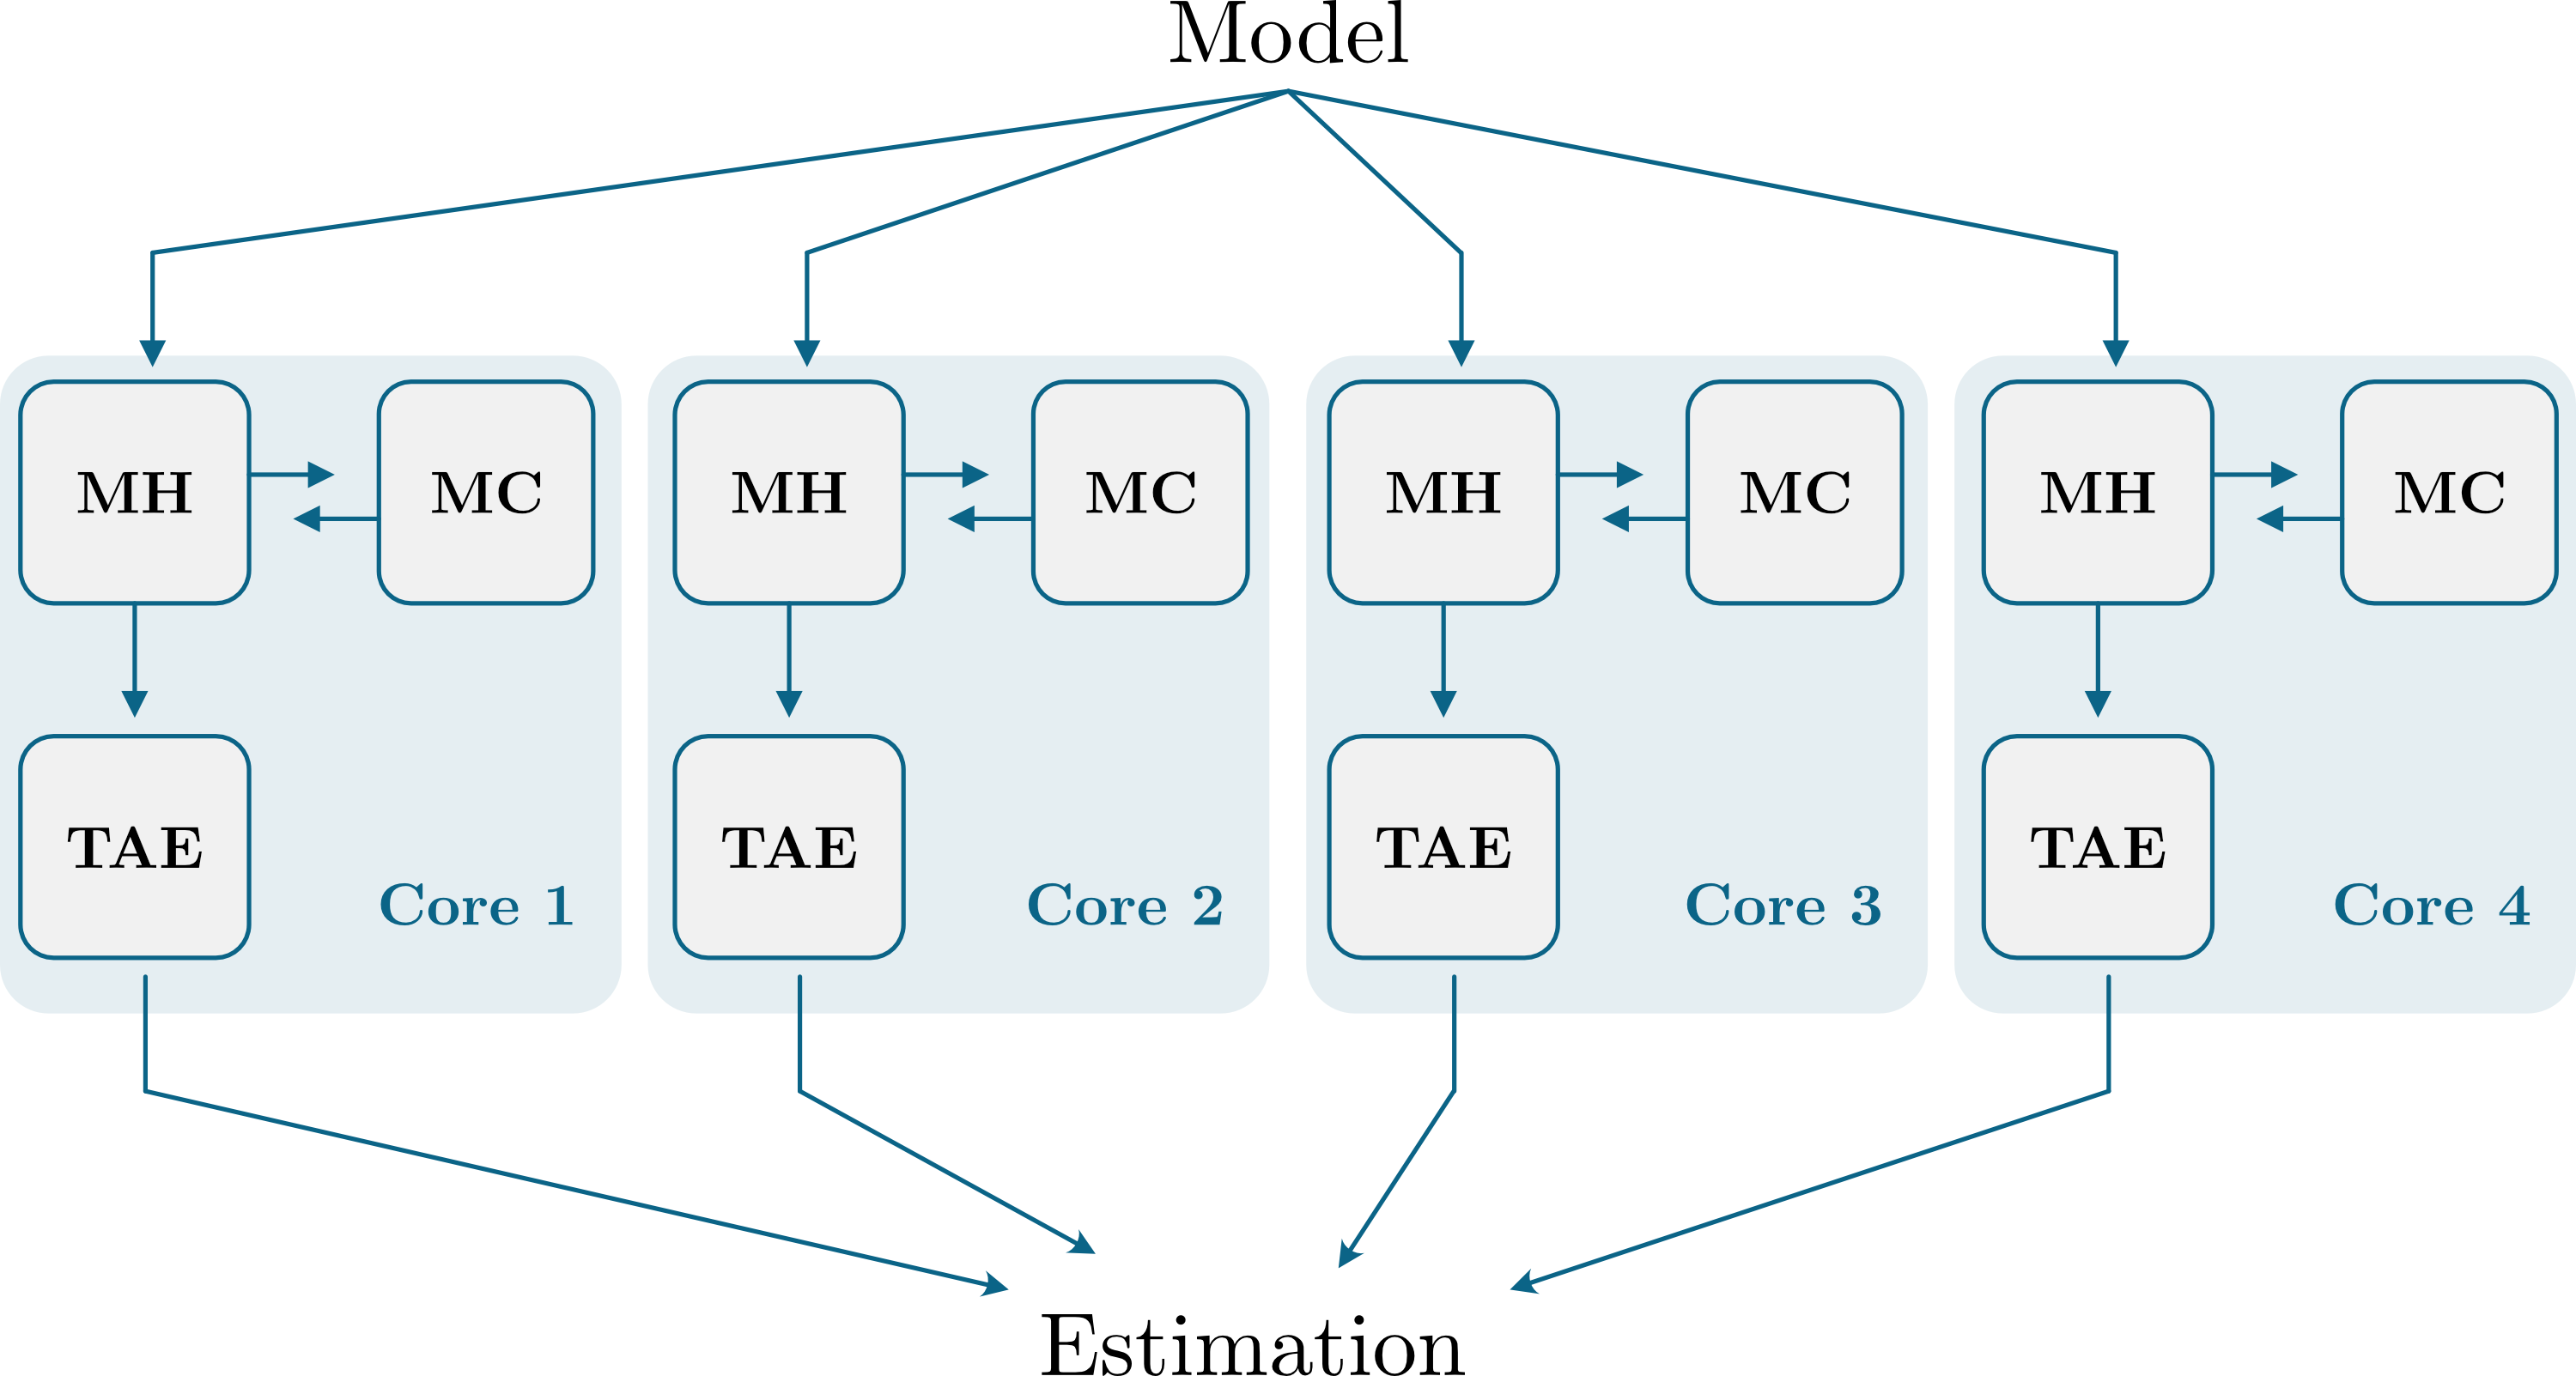
\includegraphics[width=0.95\textwidth]{img/Bayes2}
		\end{center}
	\end{frame}


	\begin{frame}
		\frametitle{Study case}
		
		\begin{block}{Model}
			\begin{center}
				$ Y_i | \mu \overset{iid}{\sim} \mathcal{N}(\mu, \sigma_{obs} ^2) $\\
				
				\vspace{0.3cm}
				
				$ \mu  \sim \mathcal{N}(\mu_0, \sigma_0^2)$
				
				$\mu_0 = 38, \quad \sigma^2_0 = 4$
			\end{center}
		\end{block}
		
		\begin{block}{Dataset}
			1000 samples generated from a Gaussian distribution:
			\begin{center}
				$
				Y_{obs} \sim \mathcal{N}(\mu_{obs}, \sigma_{obs} ^2)
				$
				
				$
				\mu_{obs} = 43, \quad
				\sigma_{obs} ^2 = 5
				$
			\end{center}
		\end{block}
	\end{frame}

	\begin{frame}
		\frametitle{Results}
		
		{\small
			$$
				\mathcal{N}(\mu_n, \sigma^2_n), 
				\quad
				\mu_n 
					= \frac{1}{ \frac{1}{\sigma_0^2} + \frac{n}{\sigma_{obs}^2} } 
					\cdot \left(\frac{\mu_0}{\sigma_0^2} + \frac{\sum y_{obs}}{\sigma_{obs}^2}\right)
					\simeq 42.99,
				\quad
				\sigma^2_n
					= \frac{1}{ \frac{1}{\sigma_0^2} + \frac{n}{\sigma_{obs}^2} } 
					\simeq 0.025
		$$
		}
	
		\begin{minipage}{0.48\textwidth}
			\begin{center}
				{\scriptsize \textbf{Coupled chains} }
				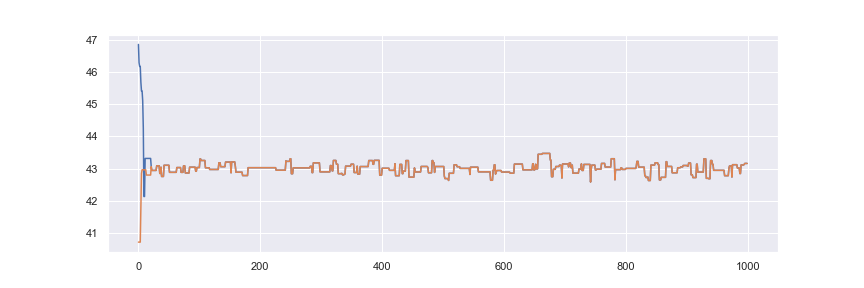
\includegraphics[width=\textwidth]{img/mcmc_coupling_chain_meeting}
			\end{center}
		\end{minipage}
		\hfill
		\begin{minipage}{0.48\textwidth}
			\begin{center}
				{\scriptsize \textbf{Complete sampling}}
				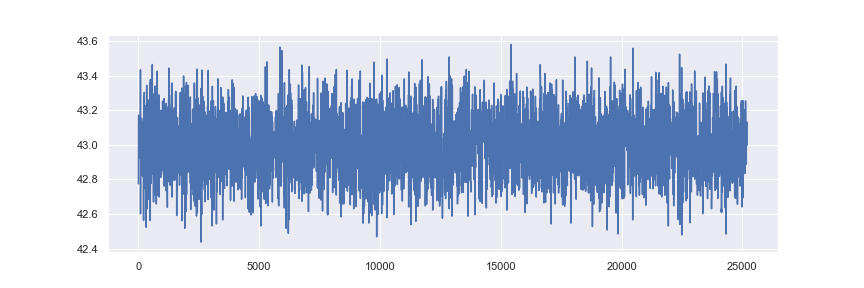
\includegraphics[width=\textwidth]{img/mcmc_coupling_sampling}
			\end{center}
		\end{minipage}
	
		\vspace{0.2cm}
	
		\begin{minipage}{0.48\textwidth}
			\begin{center}
				{\scriptsize \textbf{Sampling histogram}}
				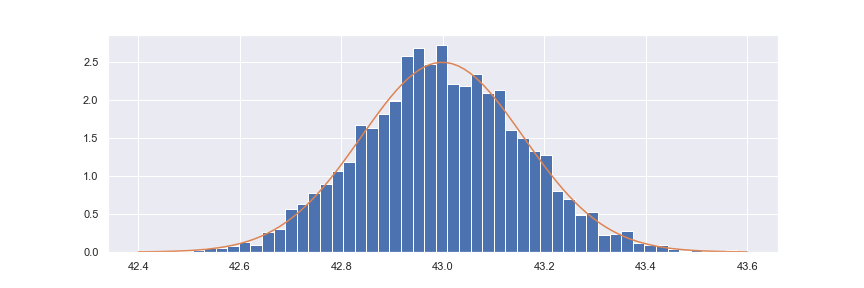
\includegraphics[width=\textwidth]{img/mcmc_coupling_histogram}
			\end{center}
		\end{minipage}
		\hfill
		\begin{minipage}{0.48\textwidth}
			\begin{center}
				{\small\textbf{Time Averaged Estimators mean:}}
				$ \mathbb{E}[H_{k:m}(X,Y)] = 42.9498$
			\end{center}
		\end{minipage}
		
		%\begin{itemize}
		%	\item posterior
		%	\item risultato del time averaged
		%	\item grafico catene che si incontrano
		%	\item istogramma dei samplings (sotto alla posterior)
		%\end{itemize}
	\end{frame}
	
\end{section}


\begin{section}{Approximate Bayesian Computation}
	
	\begin{frame}[plain]{}
		\sectionpage
	\end{frame}
	
	%%%% (dire quale summary statistica usata, quale distanza usata, quale kernel)
\begin{frame}{ABC Metropolis Hastings}
	\only<1> {
		\emph{Inputs:}
		\begin{itemize}
			\item a target posterior density $\pi(\theta | y_{obs}) \propto p(y_{obs}|\theta) \pi(\theta)$, consisting of a prior distribution $\pi(\theta)$ and a procedure of generating data under the model $p(y_{obs}|\theta)$;
			\item a Markov proposal density $g(\theta,\theta')$=$g(\theta' | \theta)$;
			\item an integer $N \textgreater0$;
			\item a kernel function $K_h(u)$ and a scale parameter $h > 0$;
			\item a low dimensional vector of summary statistics $s=S(y)$.
		\end{itemize}
		
		\emph{Initialise:} \\
		repeat:
		\begin{enumerate}
			\item choose an initial parameter vector $\theta^{(0)}$ from the support of $\pi(\theta)$;
			\item generate $ y^{(0)} \sim p(y|\theta ^ {(0)})$ from the model and compute summary statistics $s^{(0)}=S(y^{(0)})$, until ${K_h(\parallel s^{(0)}-s_{obs}\parallel)} >0$.
		\end{enumerate}
	}
	\only<2> {
		\emph{Sampling} for $i=1,...,N$:
		\begin{enumerate}
			\item generate candidate vector $\theta' \sim g(\theta^{(i-1)},\theta)$ from the proposal density $g$;
			\item generate $ y\,' \sim p(y|\theta')$ from the model and compute summary statistics  $s' = S(y\,')$;
			\item with probability $$\min \{ 1, \frac{K_h(\parallel s'-s_{obs}\parallel)   \pi(\theta')g(\theta',\theta^{(i-1)})}{K_h(\parallel s^{(i-1)}-s_{obs}\parallel)   \pi(\theta^{(i-1)})g(\theta^{(i-1)},\theta') } \}$$ 
			set $(\theta^{(i)},s^{(i)})=(	\theta',s')$. 
			Otherwise set  $(\theta^{(i)},s^{(i)})=(\theta^{(i-1)},s^{(i-1)})$.
		\end{enumerate}
		
		\emph{Output:}
		\begin{itemize}
			\item a set of correlated parameter vectors $\theta ^ {(1)},..., \theta ^ {(N)}$ from a Markov chain with stationary distribution $\pi_{ABC}(\theta |S_{obs})$.
		\end{itemize}
	}
	\end{frame}

	\begin{frame}
		\frametitle{Study case}
		\only<1>{
			\textbf{Summary statistic}: \\
			\begin{center}
				Sample mean
			\end{center}
			
			\textbf{Distance}: 
			\begin{center}
				2-norm of the difference.
			\end{center}   %malanobis nel multivariato
			
			\textbf{Kernel}: 
			$$
			K(u) = 
			\frac{1}{\sqrt{2\pi}} e^{-\frac{1}{2}u^2}, 
			\quad K_h(u) 
			= \frac{K(\frac u h)}{h}
			.
			$$
			%1/(np.sqrt(2*math.pi))np.exp(-1/2*u*2)
		}
		\only<2>{
			Same as previous: - DA RIVEDERE
			\begin{block}{Model}
				\begin{center}
					$ Y_i | \mu \overset{iid}{\sim} \mathcal{N}(\mu, \sigma_{obs} ^2) $\\
					
					\vspace{0.3cm}
					
					$ \mu  \sim \mathcal{N}(\mu_0, \sigma_0^2)$
					
					$\mu_0 = 38, \quad \sigma^2_0 = 4$
				\end{center}
			\end{block}
			
			\begin{block}{Dataset}
				1000 samples generated from a Gaussian distribution:
				\begin{center}
					$
					Y_{obs} \sim \mathcal{N}(\mu_{obs}, \sigma_{obs} ^2)
					$
					
					$
					\mu_{obs} = 43, \quad
					\sigma_{obs} ^2 = 5
					$
				\end{center}
			\end{block}
		}
	\end{frame}

	
	\begin{frame}{Results}
		\begin{center}
			\begin{minipage}{0.63\textwidth}
				\begin{center}
					{\scriptsize \textbf{Sampling}}
					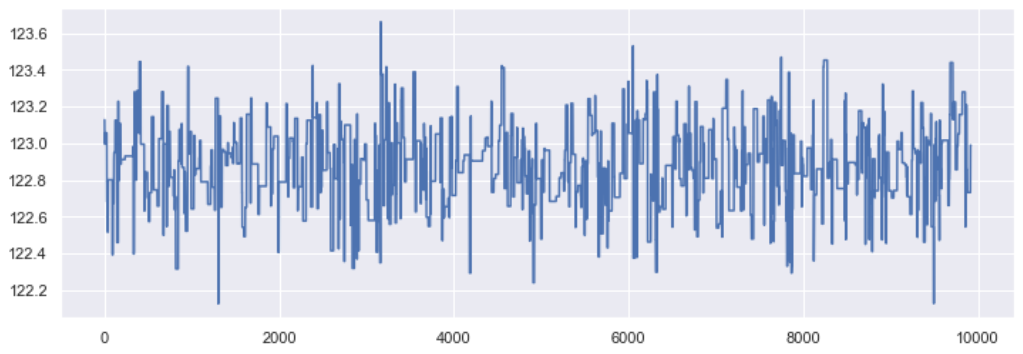
\includegraphics[width=\textwidth]{img/mcmc_abc_sampling}
				\end{center}
			\end{minipage}
		
			\vspace{0.2cm}
		
			\begin{minipage}{0.63\textwidth}
				\begin{center}
					{\scriptsize \textbf{Sampling histogram with real distribution}}
					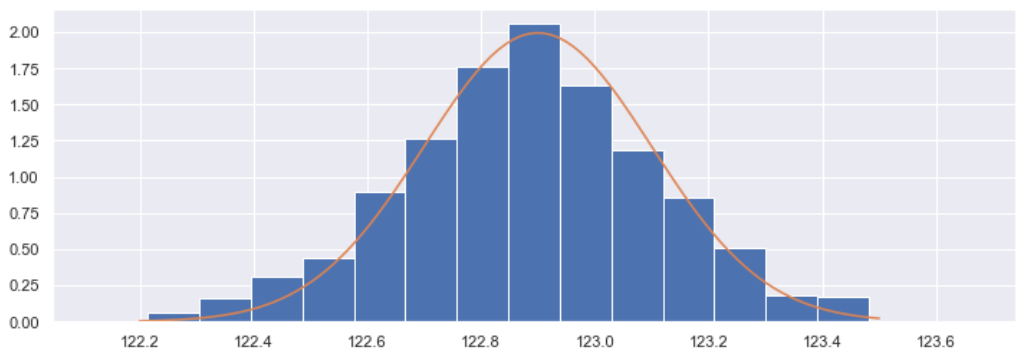
\includegraphics[width=\textwidth]{img/mcmc_abc_histogram}
				\end{center}
			\end{minipage}
		\end{center}
		% grafici per un esempio univariato con summary mean -> e uno con quantili? (funzionava?)
	\end{frame}
\end{section}

\begin{section}{The complete method: MCMC + Couplings + ABC}
	
	\begin{frame}[plain]{}
		\sectionpage
	\end{frame}

	\begin{frame}
		\frametitle{Implementation}
		\begin{center}
			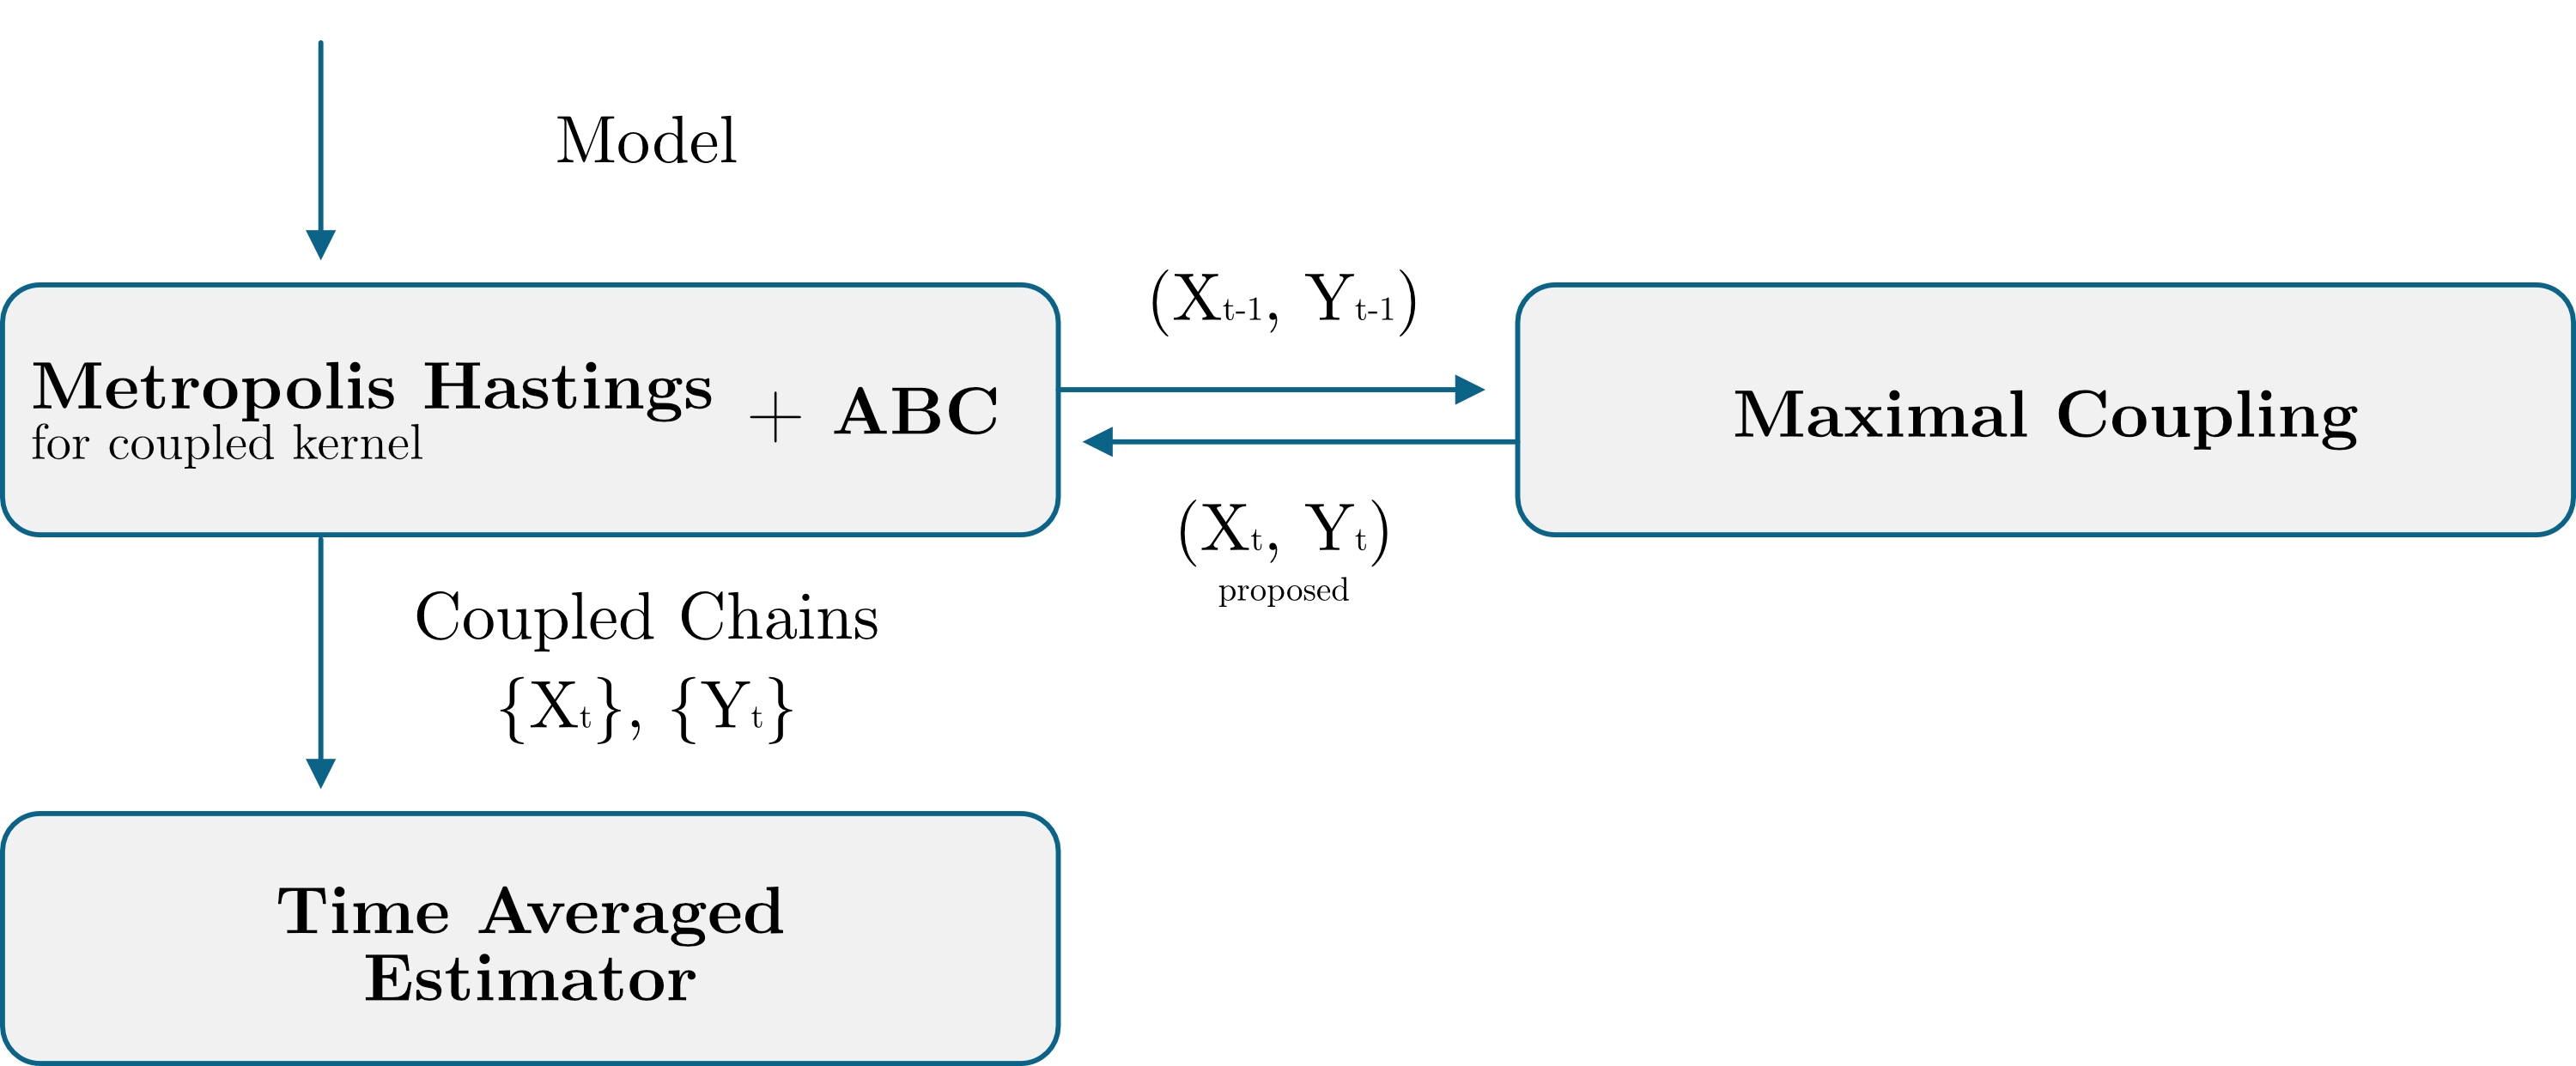
\includegraphics[width=\textwidth]{img/Bayes3}
		\end{center}
	\end{frame}

	\begin{frame}
		\frametitle{Metropolis Hastings with couplings and ABC}
		\only<1>{
			\begin{enumerate}
				\item Compute $s_{obs} = S(y_{obs})$;
				\item generate $\theta_{x}^{(0)} \sim  \pi(\mu)$ and $\theta_{y}^{(0)} \sim  \pi(\mu)$ from prior density;
				\item generate with a maximal coupling two samples of N observations such that $y_{1i} \sim \mathcal{N}(\theta_{x}^{(0)}, \sigma_{obs} ^2)$ and  $y_{2j} \sim \mathcal{N}(\theta_{y}^{(0)}, \sigma_{obs} ^2)$;
				\item compute $s_{x}^{(0)}=S(y_{1})$ and $s_{y}^{(0)}=S(y_{2})$;
				\item untill $Kh(||s_{x}^{(0)}−s_{obs}||)>0$:
				\begin{itemize}
					\item generate $\theta_{x}^{(0)} \sim  \pi(\mu)$ from prior density;
					\item generate a sample of N observations such that $y_{1i} \sim \mathcal{N}(\theta_{x}^{(0)}, \sigma_{obs} ^2)$;
					\item compute $s_{x}^{(0)}=S(y_{1})$;
				\end{itemize}
				\item untill $Kh(||s_{y}^{(0)}−s_{obs}||)>0$:
				\begin{itemize}
					\item generate $\theta_{y}^{(0)} \sim  \pi(\mu)$ from prior density;
					\item generate a sample of N observations such that $y_{2j} \sim \mathcal{N}(\theta_{y}^{(0)}, \sigma_{obs} ^2)$;
					\item compute $s_{y}^{(0)}=S(y_{2})$;
				\end{itemize}
				
			\end{enumerate}
		}
		\only<2>{
			\begin{enumerate}
				\setcounter{enumi}{7}	

				\item for i = 1,...,N:
				\begin{itemize}
					\item generate [$\theta_{x}^{(i)},\theta_{y}^{(i)}$] from a maximal coupling given [$\theta_{x}^{(i-1)},\theta_{y}^{(i-1)}$];
					\item generate from a maximal coupling two samples of N observations $y_{1} \sim p(y|\theta_{x}^{(i)})$ and $y_{2} \sim p(y|\theta_{y}^{(i)})$;
					\item compute $s_{x}^{(i)}=S(y_{1})$ and $s_{y}^{(i)}=S(y_{2})$;
					\item accept $\theta_{x}^{(i)}$ with probability 
					$$
						\frac{
							Kh(||s_{x}^{(i)}−s_{obs}||)\pi(\theta_{x}^{(i)})
						}{
							Kh(||s_{x}^{(i-1)}−s_{obs}||)\pi(\theta_{x}^{(i-1)})
						}
					$$
					and accept $\theta_{y}^{(i)}$ with probability
					$$
						\frac{
							Kh(||s_{y}^{(i)}−s_{obs}||)\pi(\theta_{y}^{(i)})
						}{
							Kh(||s_{y}^{(i-1)}−s_{obs}||)\pi(\theta_{y}^{(i-1)})
						}.
					$$ 
				\end{itemize}
			
			
			\end{enumerate}
		}
		\only<3>{
			As output we get two sets of parameter vectors: 
			$$\theta_{x}^{(1)},...,\theta_{x}^{(N)}\sim \pi_{ABC} (\theta|y_{obs});$$
			$$\theta_{y}^{(1)},...,\theta_{y}^{(N)} \sim \pi_{ABC} (\theta|y_{obs}).$$
		}
		
	
	\end{frame}

	\begin{frame}
		\frametitle{Study case}
		\only<1>{
			\textbf{Summary statistic}: \\
			\begin{center}
				Sample mean
			\end{center}
			
			\textbf{Distance}: 
			\begin{center}
				2-norm of the difference.
			\end{center}   %malanobis nel multivariato
			
			\textbf{Kernel}: 
			$$
				K(u) = 
				\frac{1}{\sqrt{2\pi}} e^{-\frac{1}{2}u^2}, 
				\quad K_h(u) 
				= \frac{K(\frac u h)}{h}
			.
			$$
			%1/(np.sqrt(2*math.pi))np.exp(-1/2*u*2)
		}
		\only<2>{
			DA SISTEMARE
			\begin{block}{Model}
				\begin{center}
					$ Y_i | \mu \overset{iid}{\sim} \mathcal{N}(\mu, \sigma_{obs} ^2) $\\
					
					\vspace{0.3cm}
					
					$ \mu  \sim \mathcal{N}(\mu_0, \sigma_0^2)$
					
					$\mu_0 = 38, \quad \sigma^2_0 = 4$
				\end{center}
			\end{block}
			
			\begin{block}{Dataset}
				1000 samples generated from a Gaussian distribution:
				\begin{center}
					$
					Y_{obs} \sim \mathcal{N}(\mu_{obs}, \sigma_{obs} ^2)
					$
					
					$
					\mu_{obs} = 43, \quad
					\sigma_{obs} ^2 = 5
					$
				\end{center}
			\end{block}
		}
	\end{frame}



	\begin{frame}
		\frametitle{Results}
		\begin{center}
			\begin{minipage}{0.63\textwidth}
				\begin{center}
					{\scriptsize \textbf{Sampling}}
					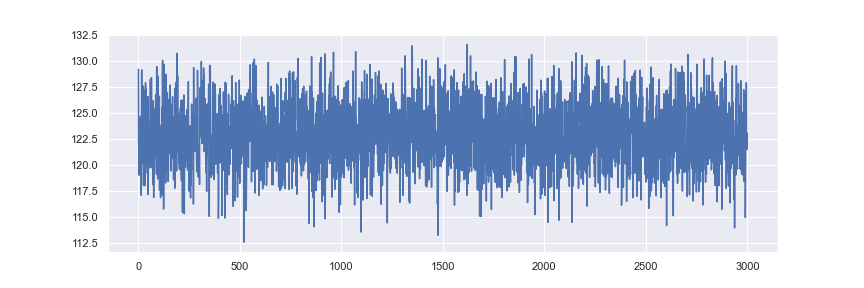
\includegraphics[width=\textwidth]{img/mcmc_couplings_abc_sampling}
				\end{center}
			\end{minipage}
			
			\vspace{0.2cm}
			
			\begin{minipage}{0.63\textwidth}
				\begin{center}
					{\scriptsize \textbf{Sampling histogram with real distribution}}
					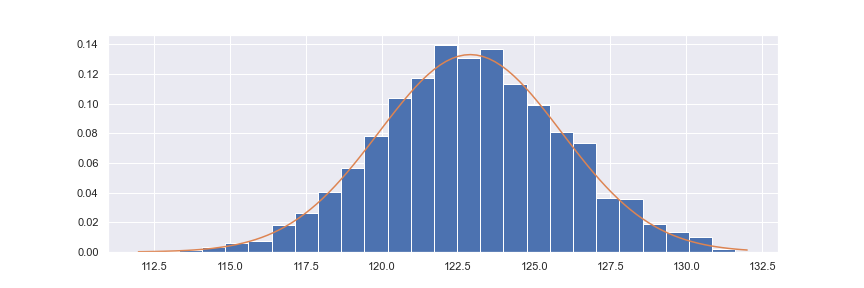
\includegraphics[width=\textwidth]{img/mcmc_couplings_abc_histogram}
				\end{center}
			\end{minipage}
		\end{center}
	\end{frame}


\end{section}


\begin{section}{Conclusions}
	
    \begin{frame}[plain]{}
		\sectionpage
	\end{frame}

	\begin{frame}{Next steps}
	
		The next step will be the conclusion of the \textbf{multivariate implementation} the MCMC with couplings and approximate bayesian computation.
		
		\vspace{0.5 cm}
		Further steps will be testing on more complex data.
	\end{frame}

	\begin{frame}{Bibliography}
		\nocite{*}
		\bibliographystyle{unsrt}
		\tiny{ \bibliography{refs_MCMC,refs_ABC} }

	
%				\begin{minipage}[t]{0.4\textwidth}
%			\footnotesize {Unbiased Markov chain Monte Carlo methods with couplings:}
%			\tiny { \bibliography{refs_MCMC} }
%		\end{minipage}
%		\hfill
%		\begin{minipage}[t]{0.4\textwidth}
%			\footnotesize {Approximate Bayesian computation:}
%			\tiny { \bibliography{refs_ABC} }
%		\end{minipage}

	\end{frame}
\end{section}

\end{document}
